\documentclass[10pt,twocolumn,letterpaper]{article}
%% Welcome to Overleaf!
%% If this is your first time using LaTeX, it might be worth going through this brief presentation:
%% https://www.overleaf.com/latex/learn/free-online-introduction-to-latex-part-1

%% Researchers have been using LaTeX for decades to typeset their papers, producing beautiful, crisp documents in the process. By learning LaTeX, you are effectively following in their footsteps, and learning a highly valuable skill!

%% The \usepackage commands below can be thought of as analogous to importing libraries into Python, for instance. We've pre-formatted this for you, so you can skip right ahead to the title below.

%% Language and font encodings
\usepackage[english]{babel}
\usepackage[utf8x]{inputenc}
\usepackage[T1]{fontenc}

%% Sets page size and margins
\usepackage[a4paper,top=2cm,bottom=2cm,left=1cm,right=1cm]{geometry}

%% Useful packages
\usepackage{amsmath}
\usepackage{graphicx}
\usepackage[colorinlistoftodos]{todonotes}
\usepackage[colorlinks=true, allcolors=blue]{hyperref}
\usepackage{natbib}
\bibliographystyle{unsrt}
%% Title
\title{
		\usefont{OT1}{bch}{b}{n}
		\huge Analyzing the Efficacy of a Small BERT Model for Part-of-Speech Tagging \\
}
\selectlanguage{english}
\usepackage{authblk}
\author[1]{Tyler Dinh}
\affil[1]{Washington University in St. Louis}

\begin{document}
\maketitle

\section{Introduction}

Part-of-speech (POS) tagging is one of the foundational tasks in Natural Language Processing (NLP), involving the labeling of every word in a sentence with its grammatical category. While classical rule-based and statistical taggers have existed for decades, modern Transformers approaches like the bidirectional, encoder-only BERT model have shown improved performance on POS tagging tasks. This project will fine-tune a small, pretrained BERT model to perform POS tagging on English text, and then conduct a linguistic analysis of where and why the model makes errors.

The data will be sourced from the Brown corpus, available directly through the NLTK package \cite{nltk_corpus}, which contains approximately one million words annotated with POS tags. This corpus will be split into a 80\%/20\% train-test split following standard machine learning practices. The model will be DistilBERT, a 40\% smaller size and 60\% faster runtime spin of BERT that is available through Hugging Face’s Transformers package. As a BERT family model, it can be fine-tuned as a token classification model for POS tagging tasks. The fine-tuned DistilBERT model will be publicly released on Hugging Face, allowing it to be easily used for evaluation on the test split in a Jupyter Notebook without needing to locally fine-tune it yourself.

The computational component involves setting up the data pipeline, tokenizing the corpus in a way that preserves word-to-tag alignment, fine-tuning the model, and evaluating with standard metrics including a classification report for each tag, a confusion matrix across tag classes, and a list of common prediction errors. The linguistic component will mainly include an analysis of the model's tagging errors and a focus on ambiguous words that can function as multiple parts of speech depending on context. I will also compare the fine-tuned DistilBERT model against NLTK's perceptron model POS tagger to see what differences exist between the two approaches.

\section{Exploratory Analysis}

To understand the structure and composition of the Brown corpus, I began with exploratory data analysis. First, I downloaded the Brown corpus using NLTK. I examined the corpus by extracting all part-of-speech tagged sentences and converting them into a pandas DataFrame with the word token and its corresponding POS tag. I inspected the dataset mainly to understand how the data is structured, which is a list of lists of tuples where each inner list represents a sentence, and each tuple contains a word and its POS tag in the sentence.  

Finally, I examined the distribution of POS tags by computing the frequency of each tag across the entire corpus and visualizing the top ten and bottom ten most common tags as a horizontal bar chart. This analysis allowed me to identify potential class imbalance / wide classification issues, which is important to address before fine-tuning a model such as DistilBERT. The top ten tags are visualized in Figure \ref{fig:top_ten_ds}, and the bottom ten tags are visualized in Figure \ref{fig:bottom_ten_ds}.

\begin{figure}[!ht]
\centering
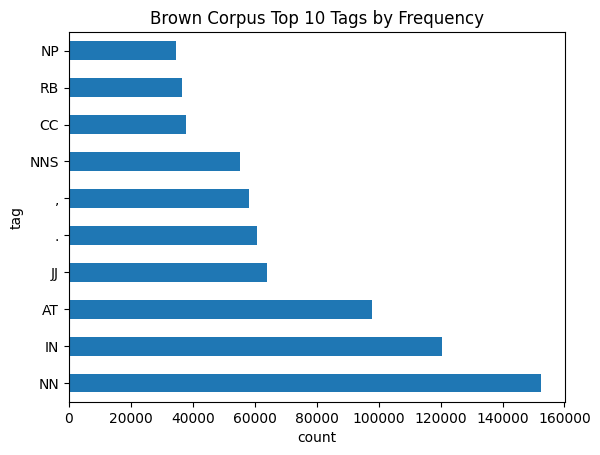
\includegraphics[width=0.4\textwidth]{figures/top_ten_ds.png}
\caption{Top ten POS tags by frequency}
\label{fig:top_ten_ds}
\end{figure}

\begin{figure}[!ht]
\centering
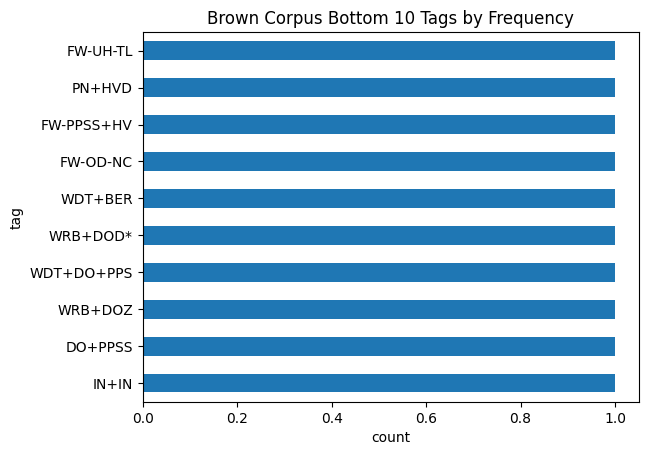
\includegraphics[width=0.4\textwidth]{figures/bottom_ten_ds.png}
\caption{Bottom ten POS tags by frequency}
\label{fig:bottom_ten_ds}
\end{figure}

\section{Methods}

The Brown corpus contains a lot of very specific POS tags. To simultaneously reduce task complexity and improve model performance for classification, I simplified the Brown corpus' tagset by extracting only the base tag. This simplification of the tagset can be justified, because the base tag should capture most of the part-of-speech information of a word, while making the classification task more manageable. This was accomplished by splitting on both the ``+'' and ``-'' characters in the tag and retaining only the first component of the tag. The simplification that I implemented reduced the number of distinct tags from the initial 472 to the simplified 105 tags.

I then extracted all tagged sentences from the Brown corpus and converted them into a structured format compatible with Hugging Face's Dataset API \cite{huggingface_datasets}. Each sentence was represented as a dictionary containing a list of word tokens and their corresponding simplified POS tags, and all of the sentences were stored inside a list. The full dataset was then split into a 80\% training and 20\% test split.

A big challenge for this project is token classification. The subword tokenization that is used by DistilBERT splits words into multiple tokens, which can potentially create a mismatch between word labels and token predictions. To address this, I implemented a method that tokenizes each sentence using DistilBERT's tokenizer with the is\_split\_into\_words=True flag to preserve word boundaries, tracks the original word that each token corresponds to using the word\_ids() method, and then finally assigns the POS label only to the first subtoken of each word.

For the fine-tuning process, I loaded the pretrained DistilBERT model for token classification \cite{huggingface_distilbert} and set it up with the appropriate number of labels given by my simplified tagset from above. I fine-tuned the model using the Hugging Face Trainer API \cite{huggingface_trainer}, which abstracts and makes model training much easier. I trained for 3 epochs, taking about 15 minutes on my laptop. The fine-tuned model was then pushed to Hugging Face \cite{distilbert_brown_pos}, where it is publicly available.

\section{Results and Analysis}

The fine-tuning process resulted in a final loss of 0.0573 on the training set at the end of epoch 3, which was a good sign that the model has learned the motions of classifying POS tags well enough. Due to this, I knew that the model was likely ready for further evaluation.

The fine-tuned model achieved a very strong performance on the test set. Due to the large number of tags, I opted to not report the scores for each tag here (it is in the Jupyter Notebook), instead for the entire test split. The classification report for the fine-tuned model is shown in Table \ref{tab:classification_report_overall}.

\begin{table}[!ht]
\centering
\caption{Overall Classification Metrics on Test Split}
\label{tab:classification_report_overall}
\begin{tabular}{|l|c|c|c|c|}
\hline
\textbf{Metric} & \textbf{Precision} & \textbf{Recall} & \textbf{F1} & \textbf{Support} \\
\hline
Accuracy & N/A & N/A & 0.98 & 231,659 \\
Macro Avg & 0.86 & 0.85 & 0.85 & 231,659 \\
Weighted Avg & 0.98 & 0.98 & 0.98 & 231,659 \\
\hline
\end{tabular}
\end{table}

The accuracy of 0.98, F1-Macro average of 0.85, and F1-Weighted average of 0.98 over a support (test set size) of 231,659 words indicate that the fine-tuned DistilBERT model performs very well for POS tagging tasks. However, the F1-Macro average is a better overall indicator across all tags, because it takes into account class imbalance in the dataset, as some tags are more prevalent. Still, its value of 0.85 is quite strong for a POS tagging task with 105 distinct tags, and it would be likely that this score would be worse on the base tagset of the Brown corpus due to limited data points.

A confusion matrix was also generated to visualize the fine-tuned model's performance on the test split. The confusion matrix is a square matrix where the rows represent the true tags and the columns represent the predicted tags. The confusion matrix for the test split is not shown due to its unreadability (large number of tags, in the Jupyter Notebook), but note that almost all classifications are correct.

The top ten most common misclassifications are shown in Table \ref{tab:top_errors}. The most common misclassification is the model predicting a noun (NN) when the true tag is an adjective (JJ), which occurs 233 times in the test split. This could be due to the fact that some words can function as both nouns and adjectives depending on context, like the phrase "shoe shop", where a noun describes another noun. The second most common misclassification is the model predicting a noun (NN) when the true tag is a proper noun (NP), which occurs 188 times in the test split. This could be due to the fact that proper nouns can sometimes be mistaken for common nouns, especially if they are not capitalized. The pretrained model is set as the uncased version of DistilBERT, which may contribute to this error.

\begin{table}[!ht]
\centering
\caption{Top 10 Most Common POS Tagging Errors on Test Split}
\label{tab:top_errors}
\begin{tabular}{|c|c|c|}
\hline
\textbf{True Tag} & \textbf{Predicted Tag} & \textbf{Count} \\
\hline
NN & JJ & 233 \\
NP & NN & 188 \\
JJ & NN & 183 \\
NN & NP & 121 \\
QL & RB & 113 \\
RB & QL & 100 \\
VBN & VBD & 96 \\
IN & CS & 84 \\
CS & IN & 72 \\
VBD & VBN & 71 \\
\hline
\end{tabular}
\end{table}

A discussion of NLTK's PerceptronTagger \cite{nltk_perceptron} and its comparison with the fine-tuned model is included in the Jupyter Notebook, but not in this report.

\section{Conclusion}

This project and project report shows that a small BERT model like DistilBERT can be effectively fine-tuned for POS tagging tasks (and possibly other NLP tasks), achieving a very strong performance on the Brown corpus, with rare misclassifications between POS categories that may result from ambiguous words functioning as multiple parts of speech.

\newpage
\bibliography{bibliography}
\end{document}
